\documentclass[journal,12pt,twocolumn]{IEEEtran}

\usepackage{setspace}
\usepackage{gensymb}
\usepackage{standalone}
\singlespacing


\usepackage[cmex10]{amsmath}

\usepackage{amsthm}
\usepackage{mathrsfs}
\usepackage{txfonts}
\usepackage{stfloats}
\usepackage{bm}
\usepackage{cite}
\usepackage{cases}
\usepackage{subfig}

\usepackage{longtable}
\usepackage{multirow}

\usepackage{enumitem}
\usepackage{mathtools}
\usepackage{steinmetz}
\usepackage{tikz}
\usepackage{circuitikz}
\usepackage{verbatim}
\usepackage{tfrupee}
\usepackage[breaklinks=true]{hyperref}
\usepackage{graphicx}
\usepackage{tkz-euclide}

\usetikzlibrary{calc,math}
\usepackage{listings}
    \usepackage{color}                                            %%
    \usepackage{array}                                            %%
    \usepackage{longtable}                                        %%
    \usepackage{calc}                                             %%
    \usepackage{multirow}                                         %%
    \usepackage{hhline}                                           %%
    \usepackage{ifthen}                                           %%
    \usepackage{lscape}     
\usepackage{multicol}
\usepackage{chngcntr}

\DeclareMathOperator*{\Res}{Res}

\renewcommand\thesection{\arabic{section}}
\renewcommand\thesubsection{\thesection.\arabic{subsection}}
\renewcommand\thesubsubsection{\thesubsection.\arabic{subsubsection}}

\renewcommand\thesectiondis{\arabic{section}}
\renewcommand\thesubsectiondis{\thesectiondis.\arabic{subsection}}
\renewcommand\thesubsubsectiondis{\thesubsectiondis.\arabic{subsubsection}}


\hyphenation{op-tical net-works semi-conduc-tor}
\def\inputGnumericTable{}                                 %%

\lstset{
%language=C,
frame=single, 
breaklines=true,
columns=fullflexible
}
\usepackage{pdfpages}
\usepackage{pgfplots}

\begin{document}


\newtheorem{theorem}{Theorem}[section]
\newtheorem{problem}{Problem}
\newtheorem{proposition}{Proposition}[section]
\newtheorem{lemma}{Lemma}[section]
\newtheorem{corollary}[theorem]{Corollary}
\newtheorem{example}{Example}[section]
\newtheorem{definition}[problem]{Definition}

\newcommand{\BEQA}{\begin{eqnarray}}
\newcommand{\EEQA}{\end{eqnarray}}
\newcommand{\define}{\stackrel{\triangle}{=}}
\bibliographystyle{IEEEtran}
\providecommand{\mbf}{\mathbf}
\providecommand{\pr}[1]{\ensuremath{\Pr\left(#1\right)}}
\providecommand{\qfunc}[1]{\ensuremath{Q\left(#1\right)}}
\providecommand{\sbrak}[1]{\ensuremath{{}\left[#1\right]}}
\providecommand{\lsbrak}[1]{\ensuremath{{}\left[#1\right.}}
\providecommand{\rsbrak}[1]{\ensuremath{{}\left.#1\right]}}
\providecommand{\brak}[1]{\ensuremath{\left(#1\right)}}
\providecommand{\lbrak}[1]{\ensuremath{\left(#1\right.}}
\providecommand{\rbrak}[1]{\ensuremath{\left.#1\right)}}
\providecommand{\cbrak}[1]{\ensuremath{\left\{#1\right\}}}
\providecommand{\lcbrak}[1]{\ensuremath{\left\{#1\right.}}
\providecommand{\rcbrak}[1]{\ensuremath{\left.#1\right\}}}
\theoremstyle{remark}
\newtheorem{rem}{Remark}
\newcommand{\sgn}{\mathop{\mathrm{sgn}}}
\providecommand{\abs}[1]{\left\vert#1\right\vert}
\providecommand{\res}[1]{\Res\displaylimits_{#1}} 
\providecommand{\norm}[1]{\left\lVert#1\right\rVert}
%\providecommand{\norm}[1]{\lVert#1\rVert}
\providecommand{\mtx}[1]{\mathbf{#1}}
\providecommand{\mean}[1]{E\left[ #1 \right]}
\providecommand{\fourier}{\overset{\mathcal{F}}{ \rightleftharpoons}}
%\providecommand{\hilbert}{\overset{\mathcal{H}}{ \rightleftharpoons}}
\providecommand{\system}{\overset{\mathcal{H}}{ \longleftrightarrow}}
	%\newcommand{\solution}[2]{\textbf{Solution:}{#1}}
\newcommand{\solution}{\noindent \textbf{Solution: }}
\newcommand{\cosec}{\,\text{cosec}\,}
\providecommand{\dec}[2]{\ensuremath{\overset{#1}{\underset{#2}{\gtrless}}}}
\newcommand{\myvec}[1]{\ensuremath{\begin{pmatrix}#1\end{pmatrix}}}
\newcommand{\mydet}[1]{\ensuremath{\begin{vmatrix}#1\end{vmatrix}}}
\numberwithin{equation}{subsection}
\makeatletter
\@addtoreset{figure}{problem}
\makeatother
\let\StandardTheFigure\thefigure
\let\vec\mathbf
\renewcommand{\thefigure}{\theproblem}
\def\putbox#1#2#3{\makebox[0in][l]{\makebox[#1][l]{}\raisebox{\baselineskip}[0in][0in]{\raisebox{#2}[0in][0in]{#3}}}}
     \def\rightbox#1{\makebox[0in][r]{#1}}
     \def\centbox#1{\makebox[0in]{#1}}
     \def\topbox#1{\raisebox{-\baselineskip}[0in][0in]{#1}}
     \def\midbox#1{\raisebox{-0.5\baselineskip}[0in][0in]{#1}}
\vspace{3cm}
\title{Assignment 5}
\author{AVVARU BHARAT}
\maketitle
\newpage
\bigskip
\renewcommand{\thefigure}{1}
\renewcommand{\thetable}{\theenumi}
Download latex-tikz codes from 
%
\begin{lstlisting}
https://github.com/Bharat437/Matrix_Theory/tree/master/Assignment5
\end{lstlisting}
\section{\textbf{Question}}
(loney 13.8) Q. Find the value of k so that the following equation may represent pair of straight lines: 
\begin{align}
    12x^2+kxy+2y^2+11x-5y+2=0\label{eq:1.1}
\end{align}
\section{\textbf{Explanation}}

Comparing the given equation with the general equation of second degree given as below:
\begin{align}
    ax^2+2bxy+cy^2++2dx+2ey+f=0\label{eq:2.1}
\end{align}

we will get $a=12$, $b=\frac{k}{2}$, $c=2$, $d=\frac{11}{2}$, $e=-\frac{5}{2}$, $f=2$.

The general equation can be expressed as:
\begin{align}
    \vec{x}^T\vec{V}\vec{x}+2\vec{u}^T\vec{x}+f=0\label{eq:2.2}
\end{align}
where
\begin{align}
    \vec{V}=\vec{V}^T=\myvec{a & b \\ b & c}=\myvec{12 & \frac{k}{2} \\ \frac{k}{2} & 2}\label{eq:2.3}\\
    \vec{u}=\myvec{d \\ e}=\myvec{\frac{11}{2} \\ -\frac{5}{2}}\label{eq:2.4}
\end{align}

The given equation represents pair of straight lines if
\begin{align}
    \mydet{\vec{V} & \vec{u} \\ \vec{u}^T & f}=0\\
    \implies\label{eq:2.6}\mydet{12 & \frac{k}{2} & \frac{11}{2} \\ \frac{k}{2} & 2 & -\frac{5}{2} \\ \frac{11}{2} & -\frac{5}{2} & 2}=0
\end{align}

The matrix in \eqref{eq:2.6} must be singular matrix and in echelon form of the matrix should consist a row with all zeros.
\begin{align}
    \implies&\myvec{12 & \frac{k}{2} & \frac{11}{2} \\ \frac{k}{2} & 2 & -\frac{5}{2} \\ \frac{11}{2} & -\frac{5}{2} & 2}\\
    \implies&\myvec{24 & k & 11 \\ k & 4 & -5 \\ 11 & -5 & 4}\\
    \xleftrightarrow[]{R_2\leftarrow 24R_2-kR1}&\myvec{24 & k & 11 \\ 0 & 96-k^2 & -120-11k \\ 11 & -5 & 4}\\
    \xleftrightarrow[]{R_3\leftarrow 24R_3-11R1}&\myvec{24 & k & 11 \\ 0 & 96-k^2 & -120-11k \\ 0 & -120-11k & -25}
\end{align}
\begin{multline}
    \xleftrightarrow[]{R_3\leftarrow (96-k^2)R_3-(-120-11k)R2}\\\myvec{24 & k & 11 \\ 0 & 96-k^2 & -120-11k \\ 0 & 0 & -96k^2-2640k-16800}\label{eq:2.11}
\end{multline}

In \eqref{eq:2.11}, the elements in last row must consist all zeros. For this to happen we should find k value.
\begin{align}
    \implies-96k^2-2640k-16800=0\\
    \implies2k^2+55k+350=0\\
    \implies(10+k)(2k+35)=0\\
    \implies k=-10\nonumber\\k=-\frac{35}{2}
\end{align}

Therefore, for $k=-10$ and $k=-\frac{35}{2}$ the given equation represents pair of straight lines.

Now Lets find equation of lines for $k=-10$.

Substitute $k=-10$ in \eqref{eq:1.1}. We get equation of pair of straight lines as:
\begin{align}
    12x^2-10xy+2y^2+11x-5y+2=0
\end{align}

Comparing above equation with \eqref{eq:2.1}, we will get $a=12$, $b=-5$, $c=2$, $d=\frac{11}{2}$, $e=-\frac{5}{2}$, $f=2$.

From \eqref{eq:2.2}, \eqref{eq:2.3}, \eqref{eq:2.4} we get
\begin{align}
    \vec{V}=\vec{V}^T=\myvec{12 & -5 \\ -5 & 2}\label{eq:2.17}\\
    \vec{u}=\myvec{\frac{11}{2} \\ -\frac{5}{2}}\label{eq:2.18}
\end{align}

If $\mydet{\vec{V}}<0$ then two lines will intersect.
\begin{align}
    \mydet{\vec{V}}&=\mydet{12 & -5 \\ -5 & 2}\\
    \implies\mydet{\vec{V}}&=-1\\
    \implies\mydet{\vec{V}}&<0
\end{align}

Therefore the lines will intersect.

The equation of two lines is given by
\begin{align}
    \vec{n_1}^T\vec{x}=c_1\label{eq:2.22}\\
    \vec{n_2}^T\vec{x}=c_2\label{eq:2.23}
\end{align}

Equating their product with \eqref{eq:2.2}
\begin{multline}
    (\vec{n_1}^T\vec{x}-c_1)(\vec{n_2}^T\vec{x}-c_2)\\=\vec{x}^T\vec{V}\vec{x}+2\vec{u}^T\vec{x}+f=0
\end{multline}
\begin{align}
    \implies\vec{n_1}*\vec{n_2}&=\{a,2b,c\}=\{12,-10,2\}\label{eq:conv}\\
    c_2\vec{n_1}+c_1\vec{n_2}&=-2\vec{u}=-2\myvec{\frac{11}{2} \\ -\frac{5}{2}}\label{eq:2.26}\\
    c_1c_2&=f=2
\end{align}

The slopes of the lines are given by roots of equation
\begin{align}
    cm^2+2bm+a=0\label{eq:poly}\\
    \implies 2m^2-10m+12=0\\
    m_i=\frac{-b\pm{\sqrt{-\mydet{\vec{V}}}}}{c}\\
    \implies m_i=\frac{5\pm{\sqrt{1}}}{2}\\
    \implies m_1=3\\
     m_2=2
\end{align}

The normal vector for two lines is given by
\begin{align}
    \vec{n_i}=k_i\myvec{-m_i\\1}\label{eq:normvec}\\
    \implies\vec{n_1}=k_1\myvec{-3\\1}\label{eq:n1}\\
    \vec{n_2}=k_2\myvec{-2\\1}\label{eq:n2}
\end{align}

Substituting \eqref{eq:n1},\eqref{eq:n2} in \eqref{eq:conv}. we get
\begin{align}
    k_1k_2=2
\end{align}

The possible combinations of ($k_1$,$k_2$) are (1,2), (2,1), (-1,-2) and (-2,-1).

lets assume $k_1=1$,$k_2=2$ we get
\begin{align}
    \implies\vec{n_1}=\myvec{-3\\1}\label{soln1}\\
    \vec{n_2}=\myvec{-4\\2}\label{soln2}
\end{align}
\begin{figure}[ht!]
    \centering
    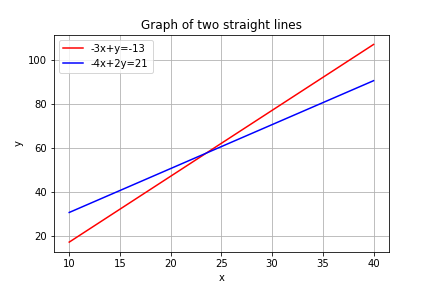
\includegraphics[width=\columnwidth]{Figure1}
    \caption{Pair of straight lines for $k=-10$}
    \label{fig:figure1}
\end{figure}

Substitute \eqref{soln1}, \eqref{soln2} in \eqref{eq:2.26} we get 
\begin{align}
    c_2\myvec{-3\\1}+c_1\myvec{-4\\2}=\myvec{ -11\\ -5}\\
    -4c_1-3c_2=-11\label{1}\\
    2c_1+c_2=-5\label{2}
\end{align}

Solving equations \eqref{1} ,\eqref{2} we get 
\begin{align}
    c_1&=-13\label{c1}\\
    c_2&=21\label{c2}
\end{align}

Substituting \eqref{soln1},\eqref{soln2},\eqref{c1},\eqref{c2} in \eqref{eq:2.22} and \eqref{eq:2.23}. We get equation of two straight lines.
\begin{align}
    \myvec{-3 & 1}\vec{x}=-13\\
    \myvec{-4 & 2}\vec{x}=21
\end{align}

The plot of these two lines is shown in Fig.~\ref{fig:figure1}.

Now Lets find equation of lines for $k=-\frac{35}{2}$.

Substitute $k=-\frac{35}{2}$ in \eqref{eq:1.1}. We get equation of pair of straight lines as:
\begin{align}
    12x^2-\frac{35}{2}xy+2y^2+11x-5y+2=0
\end{align}

Comparing above equation with \eqref{eq:2.1}, we will get $a=12$, $b=-\frac{35}{4}$, $c=2$, $d=\frac{11}{2}$, $e=-\frac{5}{2}$, $f=2$.

From \eqref{eq:2.2}, \eqref{eq:2.3}, \eqref{eq:2.4} we get
\begin{align}
    \vec{V}=\vec{V}^T=\myvec{12 & -\frac{35}{4} \\ -\frac{35}{4} & 2}\label{eq:2.48}\\
    \vec{u}=\myvec{\frac{11}{2} \\ -\frac{5}{2}}\label{eq:2.49}
\end{align}

If $\mydet{\vec{V}}<0$ then two lines will intersect.
\begin{align}
    \mydet{\vec{V}}&=\mydet{12 & -\frac{35}{4} \\ -\frac{35}{4} & 2}\\
    \implies\mydet{\vec{V}}&=-\frac{841}{16}\\
    \implies\mydet{\vec{V}}&<0
\end{align}

Therefore the lines will intersect.

Now from \eqref{eq:conv},
\begin{align}
    \implies\vec{n_1}*\vec{n_2}&=\{a,2b,c\}=\{12,-\frac{35}{2},2\}\label{eq:conv2}
\end{align}

The slopes of the lines are given by roots of equation \eqref{eq:poly}
\begin{align}
    \implies 2m^2-\frac{35}{2}m+12=0\\
    m_i=\frac{-b\pm{\sqrt{-\mydet{\vec{V}}}}}{c}\\
    \implies m_i=\frac{\frac{35}{4}\pm{\sqrt{\frac{841}{16}}}}{2}\\
    \implies m_1=8\\
     m_2=\frac{3}{4}
\end{align}

The normal vector for two lines is given by \eqref{eq:normvec}
\begin{align}
    \implies\vec{n_1}=k_1\myvec{-8\\1}\label{eq:n3}\\
    \vec{n_2}=k_2\myvec{-\frac{3}{4}\\1}\label{eq:n4}
\end{align}

Substituting \eqref{eq:n3},\eqref{eq:n4} in \eqref{eq:conv2}. we get
\begin{align}
    k_1k_2=2
\end{align}

The possible combinations of ($k_1$,$k_2$) are (1,2), (2,1), (-1,-2) and (-2,-1).

lets assume $k_1=1$,$k_2=2$ we get
\begin{align}
    \implies\vec{n_1}=\myvec{-8\\1}\label{soln3}\\
    \vec{n_2}=\myvec{-\frac{3}{2}\\2}\label{soln4}
\end{align}
\renewcommand{\thefigure}{2}
\begin{figure}[ht!]
    \centering
    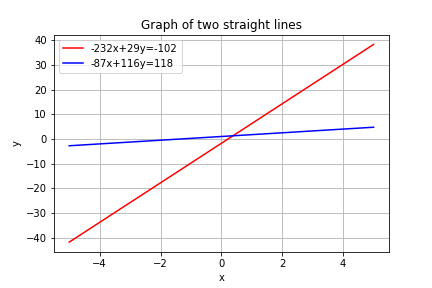
\includegraphics[width=\columnwidth]{Figure2}
    \caption{Pair of straight lines for $k=-\frac{35}{2}$}
    \label{fig:figure2}
\end{figure}

Substitute \eqref{soln3}, \eqref{soln4} in \eqref{eq:2.26} we get 
\begin{align}
    c_2\myvec{-8\\1}+c_1\myvec{-\frac{3}{2}\\2}=\myvec{ -11\\ -5}\\
    -3c_1-16c_2=-22\label{3}\\
    2c_1+c_2=-5\label{4}
\end{align}

Solving equations \eqref{3} ,\eqref{4} we get 
\begin{align}
    c_1&=-\frac{102}{29}\label{c3}\\
    c_2&=\frac{59}{29}\label{c4}
\end{align}

Substituting \eqref{soln3},\eqref{soln4},\eqref{c3},\eqref{c4} in \eqref{eq:2.22} and \eqref{eq:2.23}. we get equation of two straight lines.
\begin{align}
    \myvec{-8 & 1}\vec{x}=-\frac{102}{29}\\
    \myvec{-\frac{3}{2} & 2}\vec{x}=\frac{59}{29}
\end{align}

The plot of these two lines is shown in Fig.~\ref{fig:figure2}.
\end{document}
